\documentclass[10pt]{beamer}

\usepackage[utf8]{inputenc}
\usepackage[italian]{babel}
\usepackage[T1]{fontenc}

\usepackage{datetime2}
\DTMsetdatestyle{ddmmyyyy}
\DTMsetup{datesep=/}

\usetheme[progressbar=frametitle]{metropolis}
\usepackage{appendixnumberbeamer}

\usepackage{booktabs}
\usepackage[scale=2]{ccicons}

\usepackage{graphicx}
\usepackage{subcaption}

\usepackage{pgfplots}
\usepgfplotslibrary{dateplot}

\usepackage{hyperref}

\usepackage{xspace}
\newcommand{\themename}{\textbf{\textsc{metropolis}}\xspace}

\title{Pydoku}
\subtitle{Un risolutore di sudoku in Python con OpenCV}
\date{\DTMDisplaydate{2022}{07}{22}{}}
\author{Simone Fidanza}
\institute{Università degli studi di Bari ``Aldo Moro''}
% \titlegraphic{\hfill\includegraphics[height=1.5cm]{logo.pdf}}

\begin{document}

\maketitle

\section[Introduzione]{Introduzione}

\begin{frame}[fragile]{Pydoku}

    Pydoku è un risolutore di sudoku che fa utilizzo di librerie come OpenCV,
    TensorFlow, Keras e NumPy. Il programma estrae le cifre dall'immagine di
    una griglia, la ricostruisce digitalmente e infine risolve il sudoku.

\end{frame}

\section{Modello}

\begin{frame}{Modello di Machine Learning}
    Il modello di Machine Learning che è stato utilizzato si ispira alla rete
    neurale LeNet5+, aggiungendo vari layers fino ad arrivare ad un totale di \(10\).

    \vfill
    \begin{figure}
        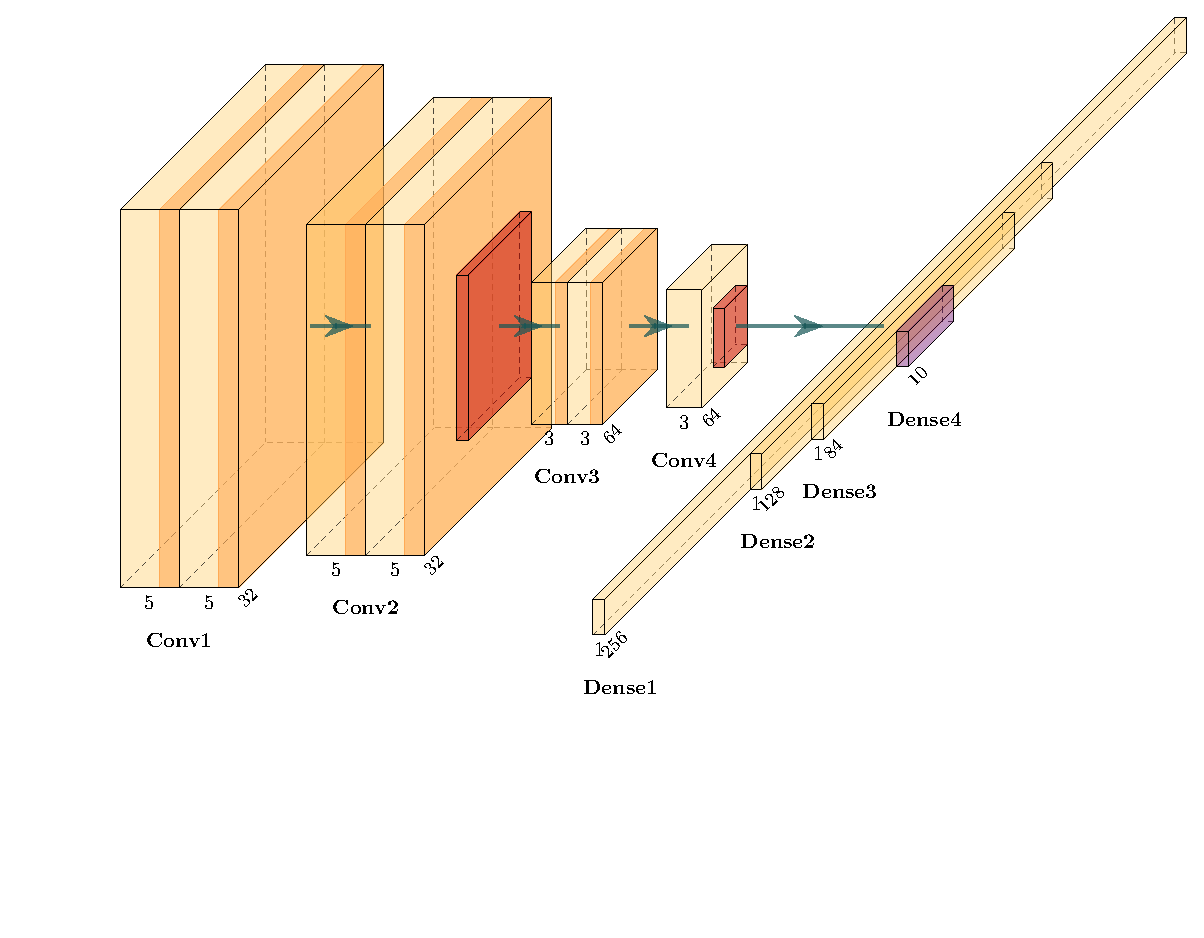
\includegraphics[width=0.9\textwidth, trim = 1cm 4.5cm 0cm 1cm]{architecture.pdf}
    \end{figure}

\end{frame}

\section{Localizzazione della griglia}

\begin{frame}[fragile]{Pre-elaborazione dell'immagine}
    Per localizzazione la griglia del sudoku è necessario pre-elaborare
    l'immagine in modo tale che essa diventi un'immagine binaria.

    \begin{figure}[h]
        \def\subwidth{0.50}
        \def\imgwidth{0.70}
        \centering
        \begin{subfigure}[b]{\subwidth\linewidth}
            \centering
            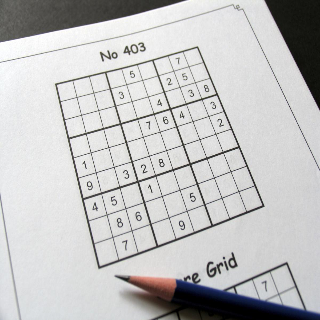
\includegraphics[width=\imgwidth\linewidth]{imgs/input.png}
            \caption{Originale}\label{subfig:input}
        \end{subfigure}%%
        \begin{subfigure}[b]{\subwidth\linewidth}
            \centering
            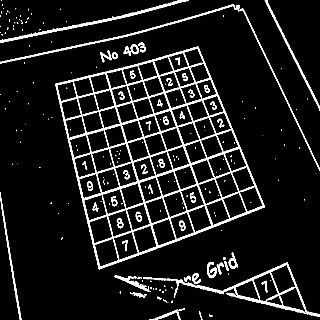
\includegraphics[width=\imgwidth\linewidth]{imgs/process_out.png}
            \caption{Pre-elaborazione}\label{subfig:preprocess}
        \end{subfigure}
    \end{figure}
\end{frame}

\begin{frame}[fragile]{Individuazione della griglia e deformazione dell'immagine}
    Per individuare la griglia è stata utilizzata la funzione \verb|cv2.findContours()|. È stato assunto che più grande dei bordi fosse la griglia
    del sudoku. Approssimando questo poligono con \verb|cv2.approxPolyDP()| sono stati ottenuti gli angoli della griglia. Usando sia
    quest'ultimi che \verb|cv2.getPerspectiveTransform()| che \verb|cv2.WarpPerspective()| l'immagine viene deformata e resa piana.

    \begin{figure}[h]
        \def\subwidth{0.50}
        \def\imgwidth{0.70}
        \centering
        \begin{subfigure}[b]{\subwidth\linewidth}
            \centering
            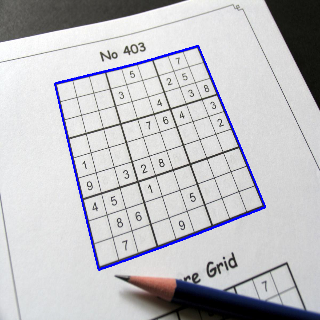
\includegraphics[width=\imgwidth\linewidth]{imgs/grid.png}
            \caption{Originale}\label{subfig:grid}
        \end{subfigure}%%
        \begin{subfigure}[b]{\subwidth\linewidth}
            \centering
            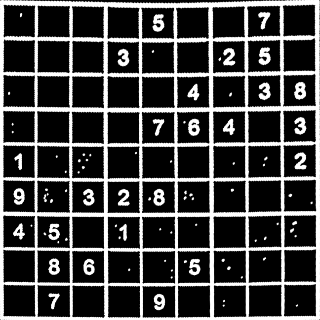
\includegraphics[width=\imgwidth\linewidth]{imgs/warp.png}
            \caption{Pre-elaborazione}\label{subfig:warp}
        \end{subfigure}
    \end{figure}
\end{frame}

\section{Analisi delle celle}

\begin{frame}[fragile]{Estrazione delle cifre}
    Per estrarre le cifre, la griglia piana viene divisa in \(81\) immagini.
    Tramite un algoritmo vengono scartate le immagini che non contengono alcun numero. Le immagini che invece ne contengono uno, vengono analizzate dalla rete neurale che effettua una predizione. In ogni caso, la cifra viene inserita in una lista.
\end{frame}

\section{Risoluzione del sudoku}

\begin{frame}[fragile]{Soluzione}
    Dopo aver ricostruito ``artificialmente'' la griglia del sudoku, questa
    viene passata all'algoritmo di risoluzione del sudoku.
    Successivamente la griglia viene mostrata a schermo.
\end{frame}

\section{Limitazioni note}

\begin{frame}[fragile]{Limitazioni}
    \begin{itemize}
        \item nel deformare e appiattire un'immagine già piana, questa viene ruotata di \(90^\circ\) in senso orario;
        \item nel determinare se una cella è priva o meno di numero, poiché l'algoritmo si basa sul numero di pixel bianchi, a volte l'algoritmo può ignorare celle che contengono dei numeri;
        \item nel predirre le cifre, la rete neurale confonde il numero \(1\) col numero \(7\) e raramente il numero \(6\) col numero \(5\) o \(8\).
    \end{itemize}
\end{frame}

\begin{frame}{Riepilogo}
    Il codice sorgente del progetto è disponibile su

    \begin{center}
        \href{https://www.github.com/sRavioli/pydoku}{github.com/sRavioli/pydoku}
    \end{center}

    Il progetto è sotto licenza \href{https://www.gnu.org/licenses/gpl-3.0.html}{GNU General Public License v3.0}.
\end{frame}

\end{document}
